\documentclass[conference]{IEEEtran}
\IEEEoverridecommandlockouts
% The preceding line is only needed to identify funding in the first footnote. If that is unneeded, please comment it out.
\usepackage{cite}
\usepackage{amsmath,amssymb,amsfonts}
\usepackage{algorithmic}
\usepackage{graphicx}
\usepackage{textcomp}
\usepackage{xcolor}
\graphicspath{{./Screenshots}}

\def\BibTeX{{\rm B\kern-.05em{\sc i\kern-.025em b}\kern-.08em
    T\kern-.1667em\lower.7ex\hbox{E}\kern-.125emX}}
\begin{document}

\title{Towards Robust Federated Learning using Knowledge Distillation Techniques\\}

\author{\IEEEauthorblockN{Arindam Jain}
\IEEEauthorblockA{School of Computing \& Augmented Intelligence \\
Arizona State University \\
ajain243@asu.edu}
\and
\IEEEauthorblockN{Kiran Sthanusubramonian}
\IEEEauthorblockA{School of Computing \& Augmented Intelligence \\
Arizona State University \\
ksthanus@asu.edu}
}

\maketitle

\section{Introduction}
With the onset of improved privacy standards, edge computing capabilities, and large-scale machine learning requirements, Federated Learning has emerged as a privacy-preserving training paradigm for localized devices without data-sharing and aggregation requirements. With privacy-preserving benefits, users of these localized devices (e.g., mobile phones) also benefit from lower latencies in terms of required responses. Potential Federated Learning applications include improved mobile computing \cite{b1}, healthcare \cite{b2}, and autonomous vehicles. 

In this project, we explore the use of Knowledge Distillation to create highly accurate and robust Federated Learning paradigms. Knowledge Distillation is conceptualized as a model compression technique in which large models with complex architectures are used to train a single smaller model that can run on devices with lesser computational capabilities while still achieving comparable performance levels. The most common Knowledge Distillation architecture is the Teacher-Student architecture (Fig.1). 

The rest of this proposal is arranged as follows: Section II will detail the findings of the Literature Survey (including potential shortcomings), Section III will highlight the Problem Statement, Section IV will discuss the Methodology (including execution plan, datasets to be used, and the metrics to evaluate \& validate the methodology), Section V will summarize the objectives and learning outcomes from this project.

\begin{figure}[htbp]
\centering
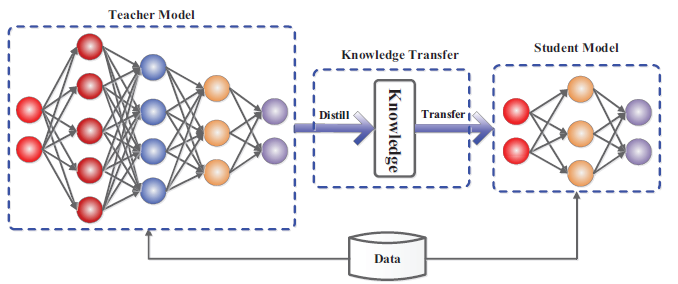
\includegraphics[scale=0.5]{Knowledge_Distillation.png}
\caption{Teacher-Student Architecture for Knowledge Distillation \cite{b3}}
\label{fig}
\end{figure}

\section{Literature Survey}

\subsection{Knowledge Distillation-based Solutions for Federated Learning}

\subsection{Improving Fairness and Robustness of Federated Learning Architectures}

\section{Problem Statement}

\section{Methodology}
\subsection{Execution Plan}
\subsection{Datasets}
\subsection{Evaluation Metrics}

\section{Objectives \& Learning Outcomes}

\begin{table}[htbp]
\caption{Table Type Styles}
\begin{center}
\begin{tabular}{|c|c|c|c|}
\hline
\textbf{Table}&\multicolumn{3}{|c|}{\textbf{Table Column Head}} \\
\cline{2-4} 
\textbf{Head} & \textbf{\textit{Table column subhead}}& \textbf{\textit{Subhead}}& \textbf{\textit{Subhead}} \\
\hline
copy& More table copy$^{\mathrm{a}}$& &  \\
\hline
\multicolumn{4}{l}{$^{\mathrm{a}}$Sample of a Table footnote.}
\end{tabular}
\label{tab1}
\end{center}
\end{table}

\begin{thebibliography}{00}
\bibitem{b1} W. Y. B. Lim et al., "Federated Learning in Mobile Edge Networks: A Comprehensive Survey," in IEEE Communications Surveys \& Tutorials, vol. 22, no. 3, pp. 2031-2063, thirdquarter 2020.
\bibitem{b2} Xu, J., Glicksberg, B.S., Su, C. et al. Federated Learning for Healthcare Informatics. J Healthc Inform Res 5, 1–19 (2021).
\bibitem{b3} Gou, J., Yu, B., Maybank, S.J. et al. Knowledge Distillation: A Survey. Int J Comput Vis 129, 1789–1819 (2021).
\bibitem{b4}
\bibitem{b5}
\bibitem{b6}
\bibitem{b7}
\end{thebibliography}

\end{document}